\begin{frame}{Linear regression}
  \begin{itemize}
    \item Estimate the associations between dependent and independent variables
    \item Predict or explain the variation in the dependent variable
    \item For instance, what is the relationship between income and annual vehicle miles traveled
  \end{itemize}
\end{frame}

\begin{frame}{Linear regression: the math}
  \Huge
  \vspace{1cm}

  \begin{equation*}
    \tikzmark{y}y = \tikzmark{a}\alpha + \tikzmark{b}\beta \tikzmark{x}x + \tikzmark{e}\epsilon
  \end{equation*}

  \begin{tikzpicture}[overlay,remember picture]
    \draw[<-] ([xshift=0.5ex, yshift=1em] pic cs:y) -- +(90:0.4cm) node[anchor=south,text=black] { \normalsize dependent variable } ;
    \draw[<-] ([xshift=0.8ex, yshift=1em] pic cs:b) -- +(90:1cm) node[anchor=south,text=black] { \normalsize coefficient } ;
    \draw[<-] ([xshift=0.5ex, yshift=1em] pic cs:e) -- +(90:0.4cm) node[anchor=south,text=black] { \normalsize error term } ;

    \draw[<-] ([xshift=0.5ex, yshift=-0.1cm] pic cs:a) -- +(270:0.5cm) node[anchor=north,text=black] { \normalsize constant } ;
    \draw[<-] ([xshift=0.5ex, yshift=-0.1cm] pic cs:x) -- +(270:1cm) node[anchor=north,text=black] { \normalsize independent variable } ;
  \end{tikzpicture}
\end{frame}

\begin{frame}{Linear regression: example}
  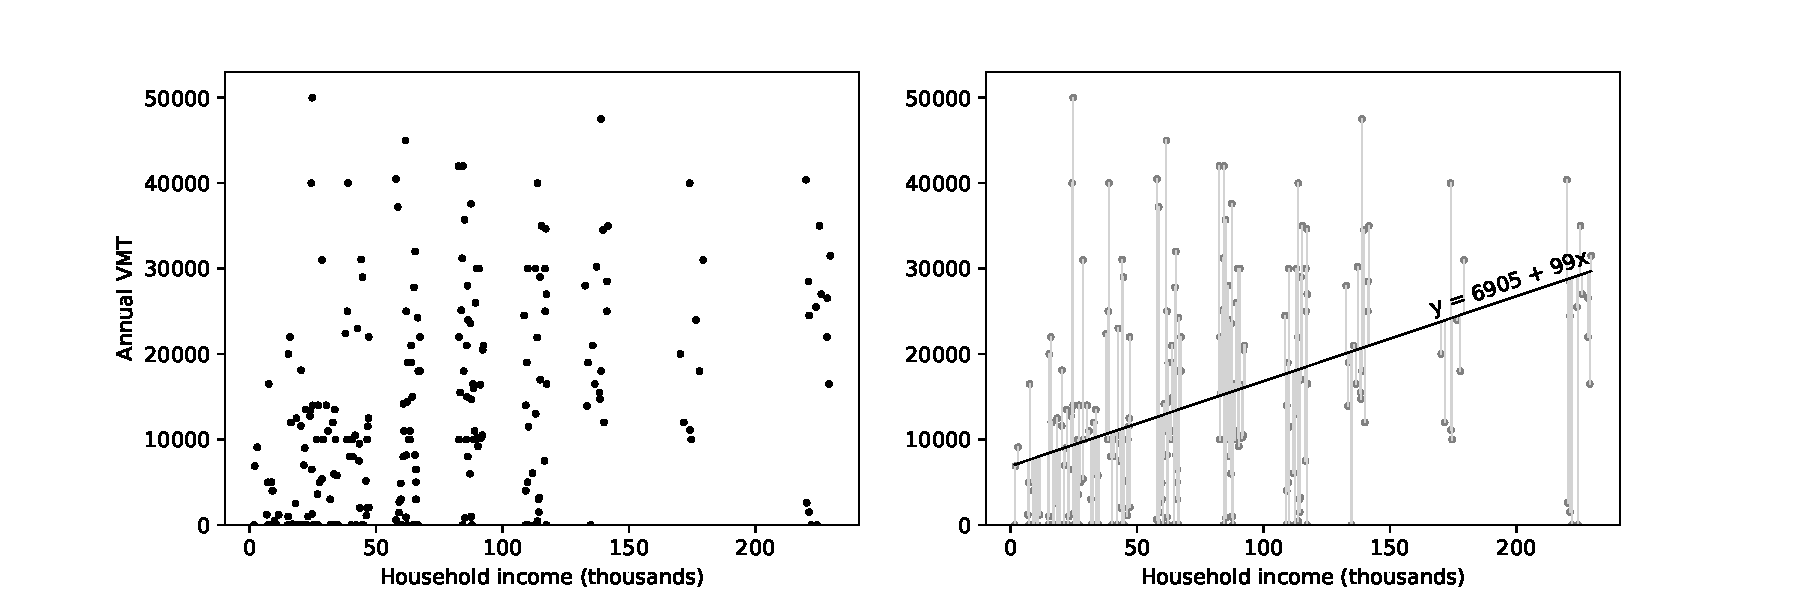
\includegraphics[width=\textwidth]{fig/bivariateregression.pdf}\\
  \tiny\citenhts
\end{frame}

\begin{frame}{Linear regression: example}
  \Huge

  \begin{equation*}
    \tikzmark{yu}y = 6905 + 99\tikzmark{xu}x
  \end{equation*}

  \begin{tikzpicture}[overlay,remember picture]
    \draw[<-] ([xshift=0.5ex, yshift=1em] pic cs:yu) -- +(90:1cm) node[anchor=south,text=black] { \normalsize annual vehicle miles traveled } ;

    \draw[<-] ([xshift=0.5ex, yshift=-0.1cm] pic cs:xu) -- +(270:1cm) node[anchor=north,text=black] { \normalsize income (thousands) } ;
  \end{tikzpicture}\\
  \tiny\citenhts
\end{frame}

\begin{frame}{Linear regression: table form}
  \small
  \begin{tabular}{lrrrrrr}
  \toprule
  {} &  Coefficient &  Std. err. &  $t$-value &  $p$-value &  95\% Conf. &   Int. \\
  \midrule
  Constant           &         6905 &       1659 &      4.161 &        0.0 &       3637 &  10173 \\
  Income (thousands) &           99 &         17 &      5.788 &        0.0 &         66 &    133 \\
  \bottomrule
  \end{tabular}
  \begin{tabular}{lclc}
  Dependent variable & \multicolumn{3}{l}{Annual vehicle miles traveled} \\
  $R^2$ & 0.12 & Adjusted $R^2$ & 0.12 \\
  Sample size & 250 && \\
  \end{tabular}\\
  \tiny\citenhts
\end{frame}

\begin{frame}{Multiple linear regression}
  \Large

  \begin{equation*}
    \tikzmark{ym}y = \tikzmark{am}\alpha + \tikzmark{b1m}\beta_1 \tikzmark{x1m}x_1 \quad + \quad \tikzmark{b2m}\beta_2 \tikzmark{x2m}x_2 \quad + \cdots + \quad \tikzmark{bnm}\beta_n \tikzmark{xnm}x_n + \tikzmark{em}\epsilon
  \end{equation*}

  \begin{tikzpicture}[overlay,remember picture]
    \draw[<-] ([xshift=0.5ex, yshift=1em] pic cs:ym) -- +(90:0.2cm) -- +(135:1.414cm) node[anchor=south,text=black] { \normalsize dependent variable } ;
    \draw[<-] ([xshift=0.8ex, yshift=1em] pic cs:b1m) -- +(90:0.5cm) node[anchor=south,text=black] { \normalsize coefficient for variable 1 } ;
    \draw[<-] ([xshift=0.8ex, yshift=1em] pic cs:b2m) -- +(90:1cm) node[anchor=south,text=black] { \normalsize coefficient for variable 2 } ;
    \draw[<-] ([xshift=0.8ex, yshift=1em] pic cs:bnm) -- +(90:0.5cm) node[anchor=south,text=black] { \normalsize coefficient for variable $n$ } ;

    \draw[<-] ([xshift=0.5ex, yshift=-0.1cm] pic cs:am) -- +(270:0.5cm) node[anchor=north,text=black] { \normalsize constant } ;
    \draw[<-] ([xshift=0.5ex, yshift=-0.1cm] pic cs:x1m) -- +(270:1cm) node[anchor=north,text=black] { \normalsize independent variable 1 } ;
    \draw[<-] ([xshift=0.5ex, yshift=-0.1cm] pic cs:x2m) -- +(270:0.5cm) node[anchor=north,text=black] { \normalsize independent variable 2 } ;
    \draw[<-] ([xshift=0.5ex, yshift=-0.1cm] pic cs:xnm) -- +(270:1cm) node[anchor=north,text=black] { \normalsize independent variable $n$ } ;
    \draw[<-] ([xshift=0.5ex, yshift=-0.1cm] pic cs:em) -- +(270:0.5cm) node[anchor=north,text=black] { \normalsize error term } ;
  \end{tikzpicture}
\end{frame}

\begin{frame}{Multiple linear regression}
  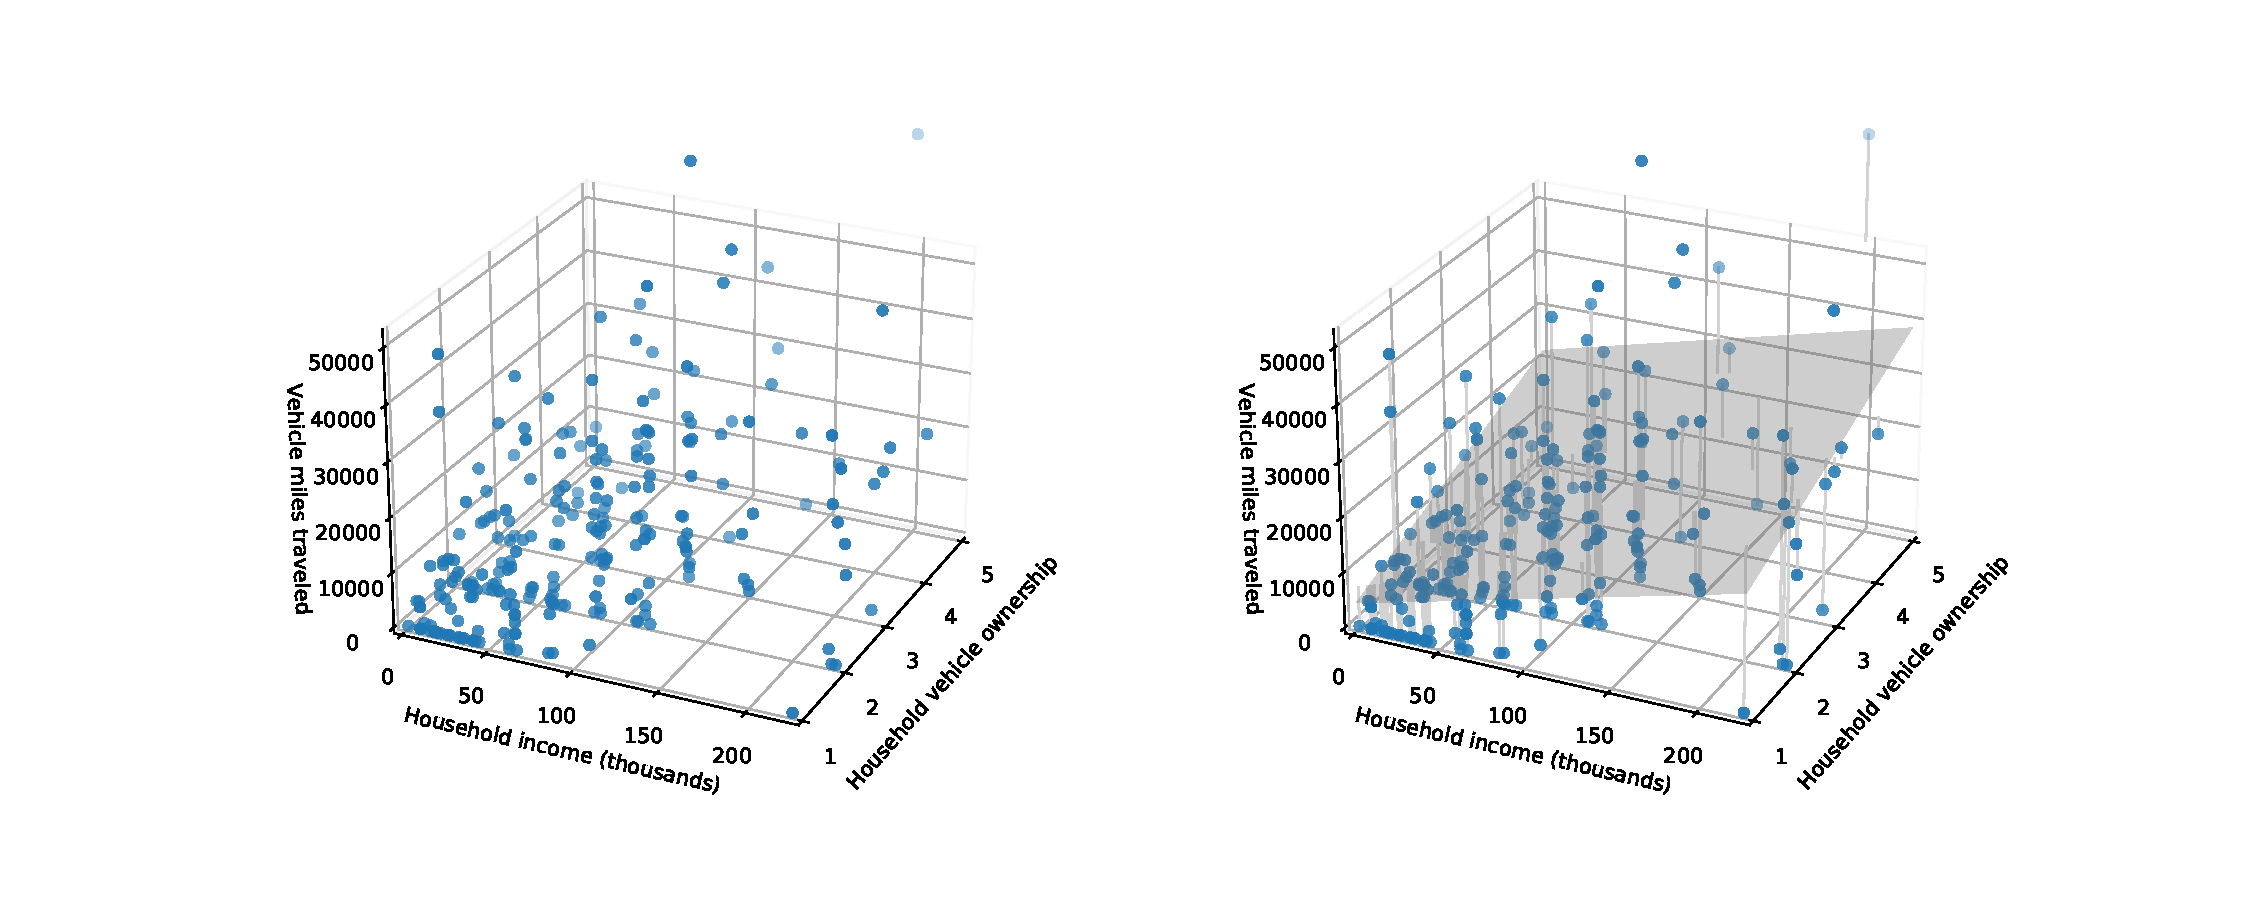
\includegraphics[width=\textwidth]{fig/trivariateregression.pdf}\\
  \tiny\citenhts
\end{frame}

\begin{frame}{Multiple linear regression}
  \small
  \begin{tabular}{lrrrrrr}
  \toprule
  {} &  Coefficient &  Std. err. &  $t$-value &  $p$-value &  95\% Conf. &  Int. \\
  \midrule
  Constant           &          -96 &       2187 &     -0.044 &      0.965 &      -4403 &  4211 \\
  Income (thousands) &           78 &         17 &      4.575 &      0.000 &         45 &   112 \\
  Number of vehicles &         4243 &        908 &      4.675 &      0.000 &       2455 &  6030 \\
  \bottomrule
  \end{tabular}
  \begin{tabular}{lclc}
  Dependent variable & \multicolumn{3}{l}{Annual vehicle miles traveled} \\
  $R^2$ & 0.19 & Adjusted $R^2$ & 0.18 \\
  Sample size & 250 && \\
  \end{tabular}\\
  \tiny\citenhts
\end{frame}

\begin{frame}{Multiple linear regression}
  \Large

  \begin{equation*}
    \tikzmark{vmt}y = -96 + \tikzmark{income}78\tikzmark{inc}x_1 \quad + \quad 4243\tikzmark{veh}x_2 + \epsilon
  \end{equation*}

  \begin{tikzpicture}[overlay,remember picture]
    \draw[<-] ([xshift=0.5ex, yshift=1em] pic cs:vmt) -- +(90:1cm) node[anchor=south,text=black] { \normalsize vehicle miles traveled } ;
    \draw[<-] ([xshift=0.8ex, yshift=1em] pic cs:veh) -- +(90:0.5cm) node[anchor=south,text=black] { \normalsize number of vehicles } ;

    \draw[<-] ([xshift=0.5ex, yshift=-0.1cm] pic cs:inc) -- +(270:0.5cm) node[anchor=north,text=black] { \normalsize income (thousands) } ;
  \end{tikzpicture}

  \pause\begin{tikzpicture}[overlay,remember picture]
    \draw[red] ([xshift=0.5em, yshift=0.5ex] pic cs:income) ellipse (0.6em and 1.5ex);
    \draw[red,->] ([xshift=0.5em, yshift=2ex] pic cs:income) -- +(55:2.5cm) node[anchor=west,text=red] { \normalsize previously 99 };
  \end{tikzpicture}

  \vspace{0.5cm}
  \tiny\citenhts
\end{frame}

\begin{frame}{Control variables}
  \begin{itemize}
    \item Every coefficient in a multiple regression model is the change in the dependent variable for a one-unit change in the independent variable, \emph{holding all other variables constant}
    \item The income coefficient now represents the association between increased income and driving, at a constant level of car ownership
    \item Often many variables in the model are \emph{control variables}
    \item The association with control variables is not of interest, but they protect the coefficients of interest from bias
  \end{itemize}
\end{frame}

% \begin{frame}{Evaluating the fit of a regression model}
%   \begin{columns}
%     \begin{column}{0.69\textwidth}
%       \begin{itemize}
%         \item $R^2$ measures the fit of a regression model
%         \item Ranges from 0 to 1
%         \item Interpretation is proportion of variance in dependent variable explained by the model
%         \item $R^2 = 0$, model is no better than predicting the mean
%         \item \alt<2>{\sout{$R^2 = 1$, model predicts perfectly} $\leftarrow$ never happens}{$R^2 = 1$, model predicts perfectly}
%         \item $R^2 = 0.42$, model explains 42\% of the variance in the dependent variable
%         \item Is high or low $R^2$ better?
%       \end{itemize}
%     \end{column}~%
%     \begin{column}{0.30\textwidth}
%       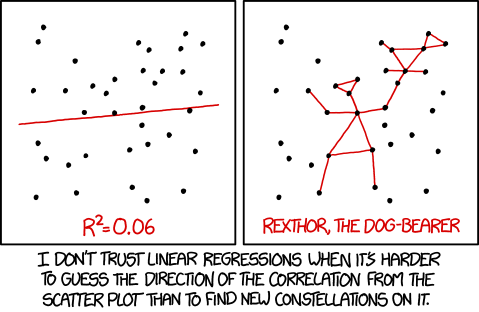
\includegraphics[width=\textwidth]{xkcd_linear_regression.png}\\
%       {\tiny \copyright~xkcd, CC BY-NC 2.5}
%     \end{column}
%   \end{columns}
% \end{frame}
%
% \begin{frame}{Evaluating the fit of a regression model}
%   \begin{columns}
%     \begin{column}{0.69\textwidth}
%       \begin{itemize}
%         \item Common alternative to $R^2$ is Adjusted $R^2$
%         \item Adding an independent variable \emph{cannot decrease} $R^2$
%         \begin{itemize}
%           \item ...even if it is meaningless
%         \end{itemize}
%         \item Adjusted $R^2$ adds a penalty for number of independent variables to prevent \emph{overfitting}
%         \item Increase in $R^2$ from additional variable must overcome this penalty
%       \end{itemize}
%     \end{column}~%
%     \begin{column}{0.3\textwidth}
%       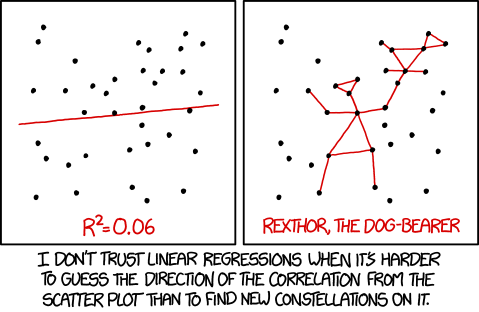
\includegraphics[width=\textwidth]{xkcd_linear_regression.png}\\
%       {\tiny \copyright~xkcd, CC BY-NC 2.5}
%     \end{column}
%   \end{columns}
% \end{frame}
%
% \begin{frame}{Evaluating the fit of a regression model}
%   \begin{columns}
%     \begin{column}{0.69\textwidth}
%       \begin{itemize}
%         \item Travel behavior models generally have $R^2$ of 0.15--0.65
%         \begin{itemize}
%           \item Smaller for models of individuals, higher for aggregate models
%         \end{itemize}
%         \item Prediction is usually not the main focus of travel behavior models
%         \item  Policy relevance, theoretical validity, and coefficient significance usually \emph{more important} than $R^2$
%       \end{itemize}
%     \end{column}~%
%     \begin{column}{0.3\textwidth}
%       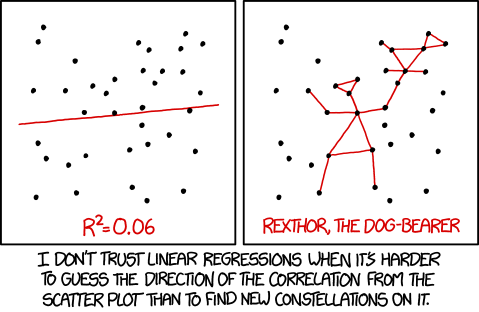
\includegraphics[width=\textwidth]{xkcd_linear_regression.png}\\
%       {\tiny \copyright~xkcd, CC BY-NC 2.5}
%     \end{column}
%   \end{columns}
% \end{frame}

\begin{frame}{Handling categorical variables in a regression}
  \begin{itemize}
    \item What if we want to include a variable with categories in a regression?
    \item For example, maybe the region where people live is associated with how much they drive
    \item What if we coded them as Northeast = 1, Midwest = 2, West = 3, South = 4?
    \pause\item Assumes that driving in the Northeast < Midwest < West < South, or vice versa
    \item Assumes that the difference from Northeast to Midwest is the same as Midwest to South
  \end{itemize}
\end{frame}

\begin{frame}{Handling categorical variables in a regression}
  \begin{itemize}
    \item The solution is to \emph{dummy variables}
    \item We create one variable for each category
    \item Set this variable to 1 if the observation is in that category, 0 otherwise
    \item Exclude one category from the regression
    \item Coefficients for other categories represent differences from excluded category
  \end{itemize}
\end{frame}

\begin{frame}{Handling categorical variables in a regression}
  \small
  \begin{tabular}{lrrrrrr}
  \toprule
  {} &  Coefficient &  Std. err. &  $t$-value &  $p$-value &  95\% Conf. &   Int. \\
  \midrule
  Constant           &        -3101 &       3109 &     -0.997 &      0.320 &      -9226 &   3024 \\
  Income (thousands) &           86 &         17 &      4.997 &      0.000 &         52 &    120 \\
  Number of vehicles &         4340 &        900 &      4.822 &      0.000 &       2567 &   6112 \\
  Region: Midwest    &         1268 &       3586 &      0.353 &      0.724 &      -5796 &   8332 \\
  Region: South      &         5229 &       2865 &      1.825 &      0.069 &       -415 &  10873 \\
  Region: West       &        -1960 &       3163 &     -0.619 &      0.536 &      -8191 &   4272 \\
  \bottomrule
  \end{tabular}
  \begin{tabular}{lclc}
  Dependent variable & \multicolumn{3}{l}{Annual vehicle miles traveled} \\
  $R^2$ & 0.23 & Adjusted $R^2$ & 0.21 \\
  Sample size & 250 && \\
  \end{tabular}\\
  \tiny\citenhts
\end{frame}

\begin{frame}{Handling categorical variables in a regression}
  \begin{equation*}
    \tikzmark{cat_ydum} y = -3101 ~+~
    86\tikzmark{cat_duminc}x_1 ~+~
    4340\tikzmark{cat_dumveh}x_2 ~+~
    \alt<1-2,4>{\textcolor{black}{1268\tikzmark{cat_dumrmw}x_3}}{\textcolor{white}{1268\tikzmark{cat_dumrmw}x_3}} ~+~
    \alt<1-4>{\textcolor{black}{5229\tikzmark{cat_dumrs}x_4}}{\textcolor{white}{5229\tikzmark{cat_dumrs}x_4}} ~-~
    \alt<1-2,4>{\textcolor{black}{1960\tikzmark{cat_dumrw}x_5}}{\textcolor{white}{1960\tikzmark{cat_dumrw}x_5}} +
    \epsilon
  \end{equation*}

  \begin{tikzpicture}[overlay,remember picture]
    \draw[<-] ([xshift=0.5ex, yshift=1em] pic cs:cat_ydum) -- +(90:0.5cm) node[anchor=south,text=black] { \scriptsize vehicle miles traveled } ;
    \draw[<-] ([xshift=0.8ex, yshift=1em] pic cs:cat_dumveh) -- +(90:0.2cm) node[anchor=south,text=black] { \scriptsize number of vehicles } ;
    \draw[<-] ([xshift=0.8ex, yshift=1em] pic cs:cat_dumrs) -- +(90:0.2cm) node[anchor=south,text=black] { \scriptsize South } ;

    \draw[<-] ([xshift=0.5ex, yshift=-0.1cm] pic cs:cat_duminc) -- +(270:0.2cm) node[anchor=north,text=black] { \scriptsize income (thousands) } ;
    \draw[<-] ([xshift=0.5ex, yshift=-0.1cm] pic cs:cat_dumrmw) -- +(270:0.5cm) node[anchor=north,text=black] { \scriptsize Midwest } ;
    \draw[<-] ([xshift=0.5ex, yshift=-0.1cm] pic cs:cat_dumrw) -- +(270:0.2cm) node[anchor=north,text=black] { \scriptsize West } ;
    \pause
    \path (pic cs:cat_ydum) -- +(225:2.25cm) node[text=black,anchor=west] {What is the estimated vehicle miles traveled for a household in the \alt<4-5>{Northeast}{South}?};
  \end{tikzpicture}\\
  \tiny\citenhts
\end{frame}
